%Version 3.1 December 2024
% See section 11 of the User Manual for version history
%
%%%%%%%%%%%%%%%%%%%%%%%%%%%%%%%%%%%%%%%%%%%%%%%%%%%%%%%%%%%%%%%%%%%%%%
%%                                                                 %%
%% Please do not use \input{...} to include other tex files.       %%
%% Submit your LaTeX manuscript as one .tex document.              %%
%%                                                                 %%
%% All additional figures and files should be attached             %%
%% separately and not embedded in the \TeX\ document itself.       %%
%%                                                                 %%
%%%%%%%%%%%%%%%%%%%%%%%%%%%%%%%%%%%%%%%%%%%%%%%%%%%%%%%%%%%%%%%%%%%%%

%%\documentclass[referee,sn-basic]{sn-jnl}% referee option is meant for double line spacing

%%=======================================================%%
%% to print line numbers in the margin use lineno option %%
%%=======================================================%%

%%\documentclass[lineno,pdflatex,bst/sn-basic]{sn-jnl}% Basic Springer Nature Reference Style/Chemistry Reference Style

%%=========================================================================================%%
%% the documentclass is set to pdflatex as default. You can delete it if not appropriate.  %%
%%=========================================================================================%%

% \documentclass[bst/sn-basic]{sn-jnl}% Basic Springer Nature Reference Style/Chemistry Reference Style
% \documentclass[Numbered,bst/sn-basic]{sn-jnl}
% \documentclass[pdflatex,Numbered,bst/sn-basic]{sn-jnl}
%%Note: the following reference styles support Namedate and Numbered referencing. By default the style follows the most common style. To switch between the options you can add or remove “Numbered” in the optional parenthesis. 
%%The option is available for: sn-basic.bst, sn-chicago.bst%  
 
%%\documentclass[pdflatex,sn-nature]{sn-jnl}% Style for submissions to Nature Portfolio journals
%%\documentclass[pdflatex,sn-basic]{sn-jnl}% Basic Springer Nature Reference Style/Chemistry Reference Style
%%\documentclass[pdflatex,bst/sn-mathphys-num]{sn-jnl}% Math and Physical Sciences Numbered Reference Style
%%\documentclass[pdflatex,sn-mathphys-ay]{sn-jnl}% Math and Physical Sciences Author Year Reference Style
%%\documentclass[pdflatex,sn-aps]{sn-jnl}% American Physical Society (APS) Reference Style
\documentclass[pdflatex,sn-vancouver-num]{sn-jnl}% Vancouver Numbered Reference Style
% \documentclass[pdflatex,sn-vancouver-ay]{sn-jnl}% Vancouver Author Year Reference Style
% \documentclass[pdflatex,sn-apa]{sn-jnl}% APA Reference Style
%%\documentclass[pdflatex,sn-chicago]{sn-jnl}% Chicago-based Humanities Reference Style

%%%% Standard Packages
%%<additional latex packages if required can be included here>

\usepackage{graphicx}%
\usepackage{multirow}%
\usepackage{amsmath,amssymb,amsfonts}%
\usepackage{amsthm}%
\usepackage{mathrsfs}%
\usepackage[title]{appendix}%
\usepackage{xcolor}%
\usepackage{textcomp}%
\usepackage{manyfoot}%
\usepackage{booktabs}%
\usepackage{algorithm}%
\usepackage{algorithmicx}%
\usepackage{algpseudocode}%
\usepackage{listings}%
%%%%

%%%%%=============================================================================%%%%
%%%%  Remarks: This template is provided to aid authors with the preparation
%%%%  of original research articles intended for submission to journals published 
%%%%  by Springer Nature. The guidance has been prepared in partnership with 
%%%%  production teams to conform to Springer Nature technical requirements. 
%%%%  Editorial and presentation requirements differ among journal portfolios and 
%%%%  research disciplines. You may find sections in this template are irrelevant 
%%%%  to your work and are empowered to omit any such section if allowed by the 
%%%%  journal you intend to submit to. The submission guidelines and policies 
%%%%  of the journal take precedence. A detailed User Manual is available in the 
%%%%  template package for technical guidance.
%%%%%=============================================================================%%%%

%% as per the requirement new theorem styles can be included as shown below
\theoremstyle{thmstyleone}%
\newtheorem{theorem}{Theorem}%  meant for continuous numbers
%%\newtheorem{theorem}{Theorem}[section]% meant for sectionwise numbers
%% optional argument [theorem] produces theorem numbering sequence instead of independent numbers for Proposition
\newtheorem{proposition}[theorem]{Proposition}% 
%%\newtheorem{proposition}{Proposition}% to get separate numbers for theorem and proposition etc.

\theoremstyle{thmstyletwo}%
\newtheorem{example}{Example}%
\newtheorem{remark}{Remark}%

\theoremstyle{thmstylethree}%
\newtheorem{definition}{Definition}%

\raggedbottom
%%\unnumbered% uncomment this for unnumbered level heads

\begin{document}

\title[Article Title]{Path Dynamics in a Deployed Path-Aware Network: Operational Measurements and Management Implications from SCIONLab}
% \title[Article Title]{Path Dynamics in a Deployed Path-Aware Network:\\A Measurement Study of SCIONLab}

%%=============================================================%%
%% GivenName	-> \fnm{Joergen W.}
%% Particle	-> \spfx{van der} -> surname prefix
%% FamilyName	-> \sur{Ploeg}
%% Suffix	-> \sfx{IV}
%% \author*[1,2]{\fnm{Joergen W.} \spfx{van der} \sur{Ploeg} 
%%  \sfx{IV}}\email{iauthor@gmail.com}
%%=============================================================%%

\author*[1,3]{\fnm{Lars} \sur{Herschbach}}\email{Lars.Herschbach@t-online.de}

\author[2,3]{\fnm{Damien} \sur{Rossi}}\email{damien.rossi@viacesi.fr}

\author[3]{\fnm{Sina} \sur{Keshvadi}}\email{skeshvadi@tru.ca}

\affil*[1]{\orgname{Goethe University Frankfurt}, \orgaddress{\street{Theodor-W.-Adorno-Platz 1}, \city{Frankfurt}, \postcode{60629}, \state{Hessen}, \country{Germany}}}

\affil[2]{\orgname{Cesi School of Engineering Toulouse}, \orgaddress{\street{16 Rue Magellan Bâtiment Alpha}, \city{Toulouse}, \postcode{31670}, \state{Labège}, \country{France}}}

\affil[3]{\orgdiv{Software Engineering}, \orgname{Thompson Rivers University}, \orgaddress{\street{805 Tru Way}, \city{Kamloops}, \postcode{V2C 0C8}, \state{British Columbia}, \country{Canada}}}

%%==================================%%
%% Sample for unstructured abstract %%
%%==================================%%

\abstract{
    Path-aware networking architectures such as SCION restore explicit, cryptographically verifiable path control to end hosts, offering greater transparency, accountability, and resilience than today's BGP-based Internet. 
    Realizing these benefits, however, demands detailed empirical knowledge of how paths behave in live deployments. 
    This paper presents the first large-scale longitudinal study of path dynamics in the operational SCIONLab testbed. 
    Deploying a measurement framework across three vantage points attached to geographically distributed SCIONLab Isolation Domains, we continuously enumerated control-plane paths and probed data-plane performance over four weeks (July–August 2025).

    Our measurements uncover three fundamental operational realities: 
    (1) substantial and frequent path-set churn, with average path lifetimes as short as 8.6 hours; 
    (2) systematic path discrepancy, in which forward and reverse path sets differ because of independent AS policies; and 
    (3) a performance trade-off whereby concurrent multipath usage increases aggregate throughput at the cost of a modest increase in the tail of jitter and a small excess of loss events, with no change in typical RTT.

    These findings challenge core assumptions of multipath transport protocols (e.g., Multipath QUIC) and define the update frequencies and directional verification requirements for automated SLA management and self-adaptive orchestration systems in path-aware networks. 
    % All measurement tools and datasets are publicly released to support reproducible research toward a Responsible Internet.
}

\keywords{Path-Aware Networking, SCION, Network Management, Network Measurement, Path Discrepancy}

%%\pacs[JEL Classification]{D8, H51}

%%\pacs[MSC Classification]{35A01, 65L10, 65L12, 65L20, 65L70}

\maketitle

\section{Introduction}~\label{sec::introduction}
    The Internet's evolution is increasingly defined by the Responsible Internet paradigm, which calls for greater transparency, accountability, and controllability in global connectivity~\cite{boldrini2024ms4pan}.
    At present, however, inter-domain routing is severely constrained by a fundamental visibility gap. 
    Traditional BGP-based routing offers endpoints almost no insight into the paths their traffic traverses and gives operators limited means to verify Service Level Agreements (SLAs) or detect disruptive route-hijacking events~\cite{giaconia2025crunching}.
    This lack of transparency forces the transport layer to treat the underlying network as a black box, selecting paths blindly and reacting slowly to inter-domain failures or congested peering links.
    
    This management blind spot has driven the development of Path-Aware Networking (PAN) architectures. 
    PAN restores explicit, cryptographically verifiable path control to end hosts and, crucially, provides Path-Verifiability, the ability to confirm that packets adhere to the intended, policy-compliant sequence of Autonomous Systems~\cite{borges2024pot}.
    By exposing path information directly to the network and transport layers, PANs supply the telemetric foundation for automated resource orchestration and intent-based traffic engineering at the edge. 
    
    Transitioning from path-oblivious to path-aware management, however, requires deep empirical ground truth. 
    Without it, autonomous rerouting risks traffic instability~\cite{jadin2022leveraging}. 
    Mechanisms such as the TCP Path Changer (TPC)~\cite{jadin2022leveraging} have shown that moving path selection to the end host is feasible with online learning, yet the practical effectiveness of such frameworks depends entirely on the stability and predictability of the underlying path dynamics.
    
    A leading realization of the path-aware vision is SCION (Scalability, Control, and Isolation on Next-Generation Networks). 
    Originally proposed as a clean-slate architecture~\cite{clark2018designing, zhang2011scion}, SCION has matured into operational deployments across academia and industry~\cite{anapaya2025}. 
    It grants endpoints explicit, cryptographically verifiable control over the exact sequence of Autonomous Systems their traffic traverses, enabling hosts to discover and orchestrate traffic across multiple, diverse, and independent end-to-end paths.
    
    This path-selection capability aligns naturally with the growing interest in multipath transport protocols. 
    Multipath TCP~\cite{rfc8684} has already demonstrated the benefits of using heterogeneous links in parallel. 
    The forthcoming Multipath QUIC~\cite{de2017multipath}, now under standardization in the IETF~\cite{ietf-quic-multipath-15}, extends this concept to QUIC's flexible, encrypted transport layer. 
    In a path-aware environment such as SCION, these protocols can exploit a much richer set of paths with greater diversity in latency, bandwidth, and reliability.
    The resulting shift of path-selection authority from core routers to end hosts fundamentally redefines traffic management~\cite{kruger2021early}: global traffic distribution now emerges directly from collective path choices made at the hosts.
    
    This decentralization, however, introduces new management challenges. 
    It creates a Cost of Multipath (CoM), the utilization penalty incurred when hosts favor redundancy over traditional shortest-path efficiency~\cite{kruger2021early, CK05}. 
    Moreover, because SCION's control plane continuously refreshes path segments through beaconing, path properties change dynamically. 
    Effective lifecycle management therefore requires moving beyond static selection toward real-time telemetry and automated scoring services. 
    These observations raise critical operational questions: Are SCION-exposed paths stable enough for autonomous transport protocols to use them effectively? Are paths symmetric? Does concurrent use of many paths always improve performance, or does it introduce resource contention?
    
    To bridge this gap, this paper presents a telemetry framework and the first large-scale longitudinal study of the SCION architecture on a live path-aware network~\cite{kwon2020scionlab}. 
    We provide the empirical evidence of path churn and asymmetry necessary to define the operational boundaries and update frequencies required for automated management entities. 
    Our findings reveal a highly dynamic environment that challenges common assumptions in multipath protocol design and supplies data-driven insights for the next generation of self-adaptive transport protocols.
    
    Our main contributions are:
    \begin{enumerate}
        \item An empirical characterization of SCIONLab's path dynamics, revealing significant control-plane churn with average path lifetimes as short as 8.6 hours.
        \item The identification of \textit{path discrepancy}, a phenomenon in which routing policies create asymmetric path availability between endpoints, directly impacting bidirectional SLA verification.
        \item An analysis of the performance trade-offs in concurrent multipath usage, showing that concurrent transmission increases aggregate throughput at the cost of a modest increase in the tail of jitter and a small excess of loss events, with no change in typical RTT.
        \item The public release of a measurement suite designed for reproducible management research on path-aware architectures.
    \end{enumerate}
        
    The remainder of this paper is structured as follows. 
    Section~\ref{sec::backgroundAndRelatedwork} discusses SCION and related multipath transport work. 
    Section~\ref{sec::methodology} details our measurement methodology. 
    Section~\ref{sec::result} presents the results, Section~\ref{sec::discussion} discusses their implications, and Section~\ref{sec::conclusion} concludes.

\section{Background and Related Works}~\label{sec::backgroundAndRelatedwork}

    This section first provides the essential background on the SCION architecture, with particular emphasis on the dynamic path environment created by its beaconing process. It then situates our longitudinal study within the broader literature on path-aware networking.

\subsection{Background}~\label{subsec::background}

    SCION (Scalability, Control, and Isolation on Next-Generation Networks) is a clean-slate Internet architecture designed for high availability, security, and fine-grained path control~\cite{zhang2011scion}. Its central innovation is path awareness: end hosts can explicitly select the exact sequence of Autonomous Systems (ASes) that their packets traverse. To improve scalability and fault isolation, SCION organizes ASes into Isolation Domains (ISDs), each with its own trust roots and core ASes. Routing problems within one ISD are thus contained and do not propagate globally, while inter-ISD connectivity is handled exclusively by core ASes.

    SCION cleanly separates the control and data planes. Path discovery occurs in the control plane through a continuous \emph{beaconing} process: beacon servers in each AS generate Path Construction Beacons (PCBs). As PCBs propagate toward the ISD core, every AS appends cryptographically signed hop information, thereby creating validated path segments (Figure~\ref{fig:scion-architecture}). These segments are classified as up-segments (source AS toward its ISD core), core-segments (between ISD cores), and down-segments (remote ISD core to destination AS). End hosts combine one segment of each type to construct complete end-to-end paths. Because segments have a finite lifetime and must be refreshed by new beacons, the set of available paths is inherently dynamic~\cite{krahenbuhl2024glids}.

\begin{figure}[htbp]
  \centering
  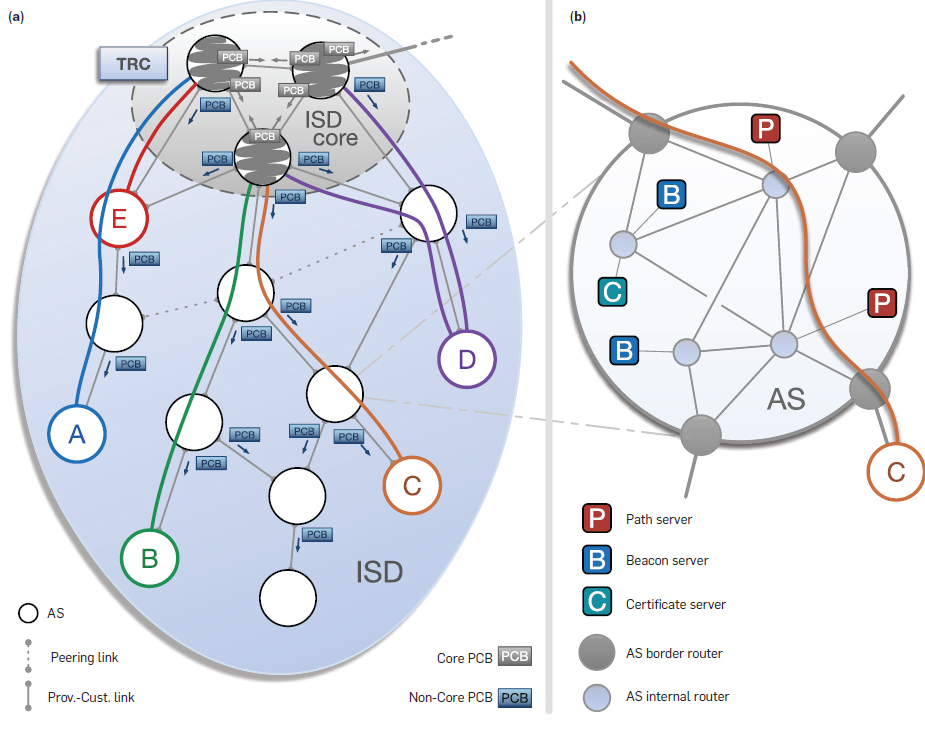
\includegraphics[width=0.8\linewidth]{figures/f2.jpg}
  \caption{SCION path construction overview (adapted from~\cite{chuat2022complete}). (a) An Isolation Domain with PCBs propagated from the ISD core and the resulting path segments from several ASes to the core. (b) Magnified view of an AS showing its routers and servers.}
  \label{fig:scion-architecture}
\end{figure}

    In the data plane, SCION employs packet-carried forwarding state (PCFS): the complete inter-domain path, including ingress and egress interfaces, is embedded in every packet header. This enables stateless forwarding between ASes and eliminates the need for large inter-domain routing tables.

    For multipath transport, SCION therefore offers both opportunities (e.g. many topologically diverse, policy-compliant paths) and challenges (e.g. a large and continuously changing path set with variable performance characteristics). Two notions of stability are particularly relevant: (1) \emph{control-plane stability}, i.e., the persistence of discoverable paths over time, and (2) \emph{data-plane stability}, i.e., the consistency of performance metrics (latency, loss, jitter) on any given path. The interplay between these two layers ultimately determines the effectiveness of multipath transport over SCION. For a comprehensive technical specification, see the SCION book~\cite{chuat2022complete} and the original architectural analysis~\cite{zhang2011scion}.


\subsection{Related Work}~\label{subsec::relatedwork}
    Research on path-aware architectures has progressed from early clean-slate designs to practical questions of automated orchestration and empirical validation of host-driven networking.
    A foundational line of work examines how inter-domain routing policies affect path availability and stability. Koole and Pawlus~\cite{koole2023comparative} compared routing policies in BGP versus SCION and showed that SCION's explicit policy mechanisms improve path stability, diversity, and resilience. Complementing this, Kr{\"a}henb{\"u}hl et al.~\cite{krahenbuhl2021deployment} evaluated the deployment and scalability of SCION's inter-domain multipath routing infrastructure, demonstrating that its path-construction algorithms can achieve near-optimal path diversity. Together, these studies supply the theoretical performance bounds that our longitudinal measurements assess under real-world operating conditions.

    As path-selection authority shifts from core routers to end hosts, attention has turned to automated management systems that hide architectural complexity from applications. Boldrini et al.~\cite{boldrini2024ms4pan} introduced MS4PAN, a database-centric framework that stores real-time probes and applies multi-objective optimization to select paths satisfying strict Service Level Agreements (SLAs). Similarly, Kr{\"u}ger et al.~\cite{kruger2023path} proposed the Path Oracle, a management service that aggregates end-to-end telemetry into actionable path scores. In contrast to traditional server-driven approaches such as the Application-Layer Traffic Optimization (ALTO) protocol~\cite{rfc7285}, the Path Oracle maintains a link-level Network View derived from donated measurements, enabling applications to adapt to dynamic loads without per-flow probing. The authors emphasize, however, that the utility of such scoring services depends critically on the freshness of the underlying data. Our study supplies the empirical characterization of path churn and asymmetry that defines the required update frequencies and operational boundaries for these management entities.
    
    Our work is also situated within the Responsible Internet paradigm~\cite{hesselman2020responsible}, which seeks to replace today's black-box inter-domain routing with a managed infrastructure that emphasizes transparency and accountability. Hesselman et al. envision a Network Inspection Plane (NIP) that delivers measurement-based operator descriptions to users, paired with a Network Control Plane (NCP) for high-level intent expression. While SCION supplies the foundational path-control mechanisms~\cite{zhang2011scion}, its effectiveness as a managed system hinges on the empirical stability and predictability of the underlying paths. By providing high-cadence telemetry on churn and discrepancy, our longitudinal study directly supports the NIP and supplies the ground truth required for SLA verification and automated resource orchestration.
    
    Recent advances have moved beyond path discovery toward full lifecycle service orchestration and verification. Borges et al.~\cite{borges2024pot} presented PoT-PolKA, a scalable in-situ framework that leverages IOAM for Proof-of-Transit verification without additional probe traffic. Relying on Strict Source Routing (SSR) and fixed route identifiers, PoT-PolKA enforces policy-compliant paths at the data plane. Our characterization of path dynamics complements this enforcement layer by defining how frequently PoT metadata must be refreshed to remain accurate in the presence of control-plane churn.
    
    The practical value of path-aware architectures is ultimately realized in transport protocols engineered to exploit topological diversity. John et al.~\cite{john2023dmtp} designed DMTP, a deadline-aware multipath protocol optimized for latency-sensitive traffic, while Gartner et al.~\cite{gartner2023hercules} introduced Hercules, a high-speed bulk-transfer system that harnesses path diversity for improved aggregate throughput. Although these protocols implicitly assume path stability and symmetry, our empirical results on churn and discrepancy provide the realistic operating conditions needed to evaluate and refine their performance.
    
    Finally, the SCIONLab testbed~\cite{kwon2020scionlab} has served as the primary global platform for evaluating SCION. van Rijswijk-Deij et al.~\cite{vanrijswijk2023sciontestbed} developed a benchmarking suite for production-grade metrics, and Battipaglia et al.~\cite{battipaglia2023evaluation} examined the usability of user-driven path control. While these studies deliver valuable snapshots, our four-week longitudinal campaign extends them by capturing the dynamic phenomena—path churn, discrepancy, and multipath performance trade-offs—that govern long-term protocol reliability and management effectiveness.

   \section{Measurement Methodology}~\label{sec::methodology}

    \subsection{Experimental Setup}
    To characterize the operational dynamics of a live path-aware network at scale, we designed and deployed a fully automated, distributed telemetry framework across three identical Google Cloud Platform virtual machines (VMs) provisioned as vantage-point autonomous systems (ASes) within the SCIONLab testbed. 
    The VMs were co-located in the high-performance \texttt{us-central1-a} zone to eliminate variability introduced by wide-area IP transit between vantage points. 
    Each VM attached to the SCION infrastructure through a distinct inter-domain entry point, thereby exercising independent control-plane and data-plane paths while ensuring that observed performance metrics (latency, loss, jitter, and throughput) could be attributed primarily to SCION path dynamics rather than cloud-provider artifacts. Although the three measurement VMs were deliberately co-located in the same GCP zone to remove cloud-transit variability between them, they were attached to three geographically distributed SCIONLab Isolation Domains (ISD 17/Switzerland, ISD 18/United States, and ISD 19/Europe).

    The vantage-point ASes corresponded to the production-grade SCIONLab infrastructure in ISD~17 (Switzerland), ISD~18 (United States), and ISD~19 (Europe), collectively labeled AS-1, AS-2, and AS-3 in our configuration. 
    Measurements formed a full mesh: each vantage point actively probed the other two, enabling bidirectional characterization of inter-AS path behavior. 
    An overview of the SCIONLab topology at the time of the campaign is provided in Figure~\ref{fig:scionlab-topology}. 
    Although the testbed contained additional ASes, only those reachable throughout the study were retained for longitudinal analysis.

    The measurement campaign operated continuously for four weeks (11 July–11 August 2025). 
    After an initial five-day stabilization window (11–15 July 2025), during which the newly attached vantage-point ASes completed path discovery and the control plane settled, we restricted all subsequent analysis to the stable 27-day period from 16 July to 11 August 2025. A cron-scheduled pipeline executed the entire measurement suite at 30-minute intervals on every vantage point. 
    All raw outputs were written as timestamped JSON files and automatically archived daily, createing a complete, reproducible trace of both control-plane advertisements and data-plane performance and are available~\cite{github-scionlab-data-2}.

    \begin{figure}[htbp]
      \centering
      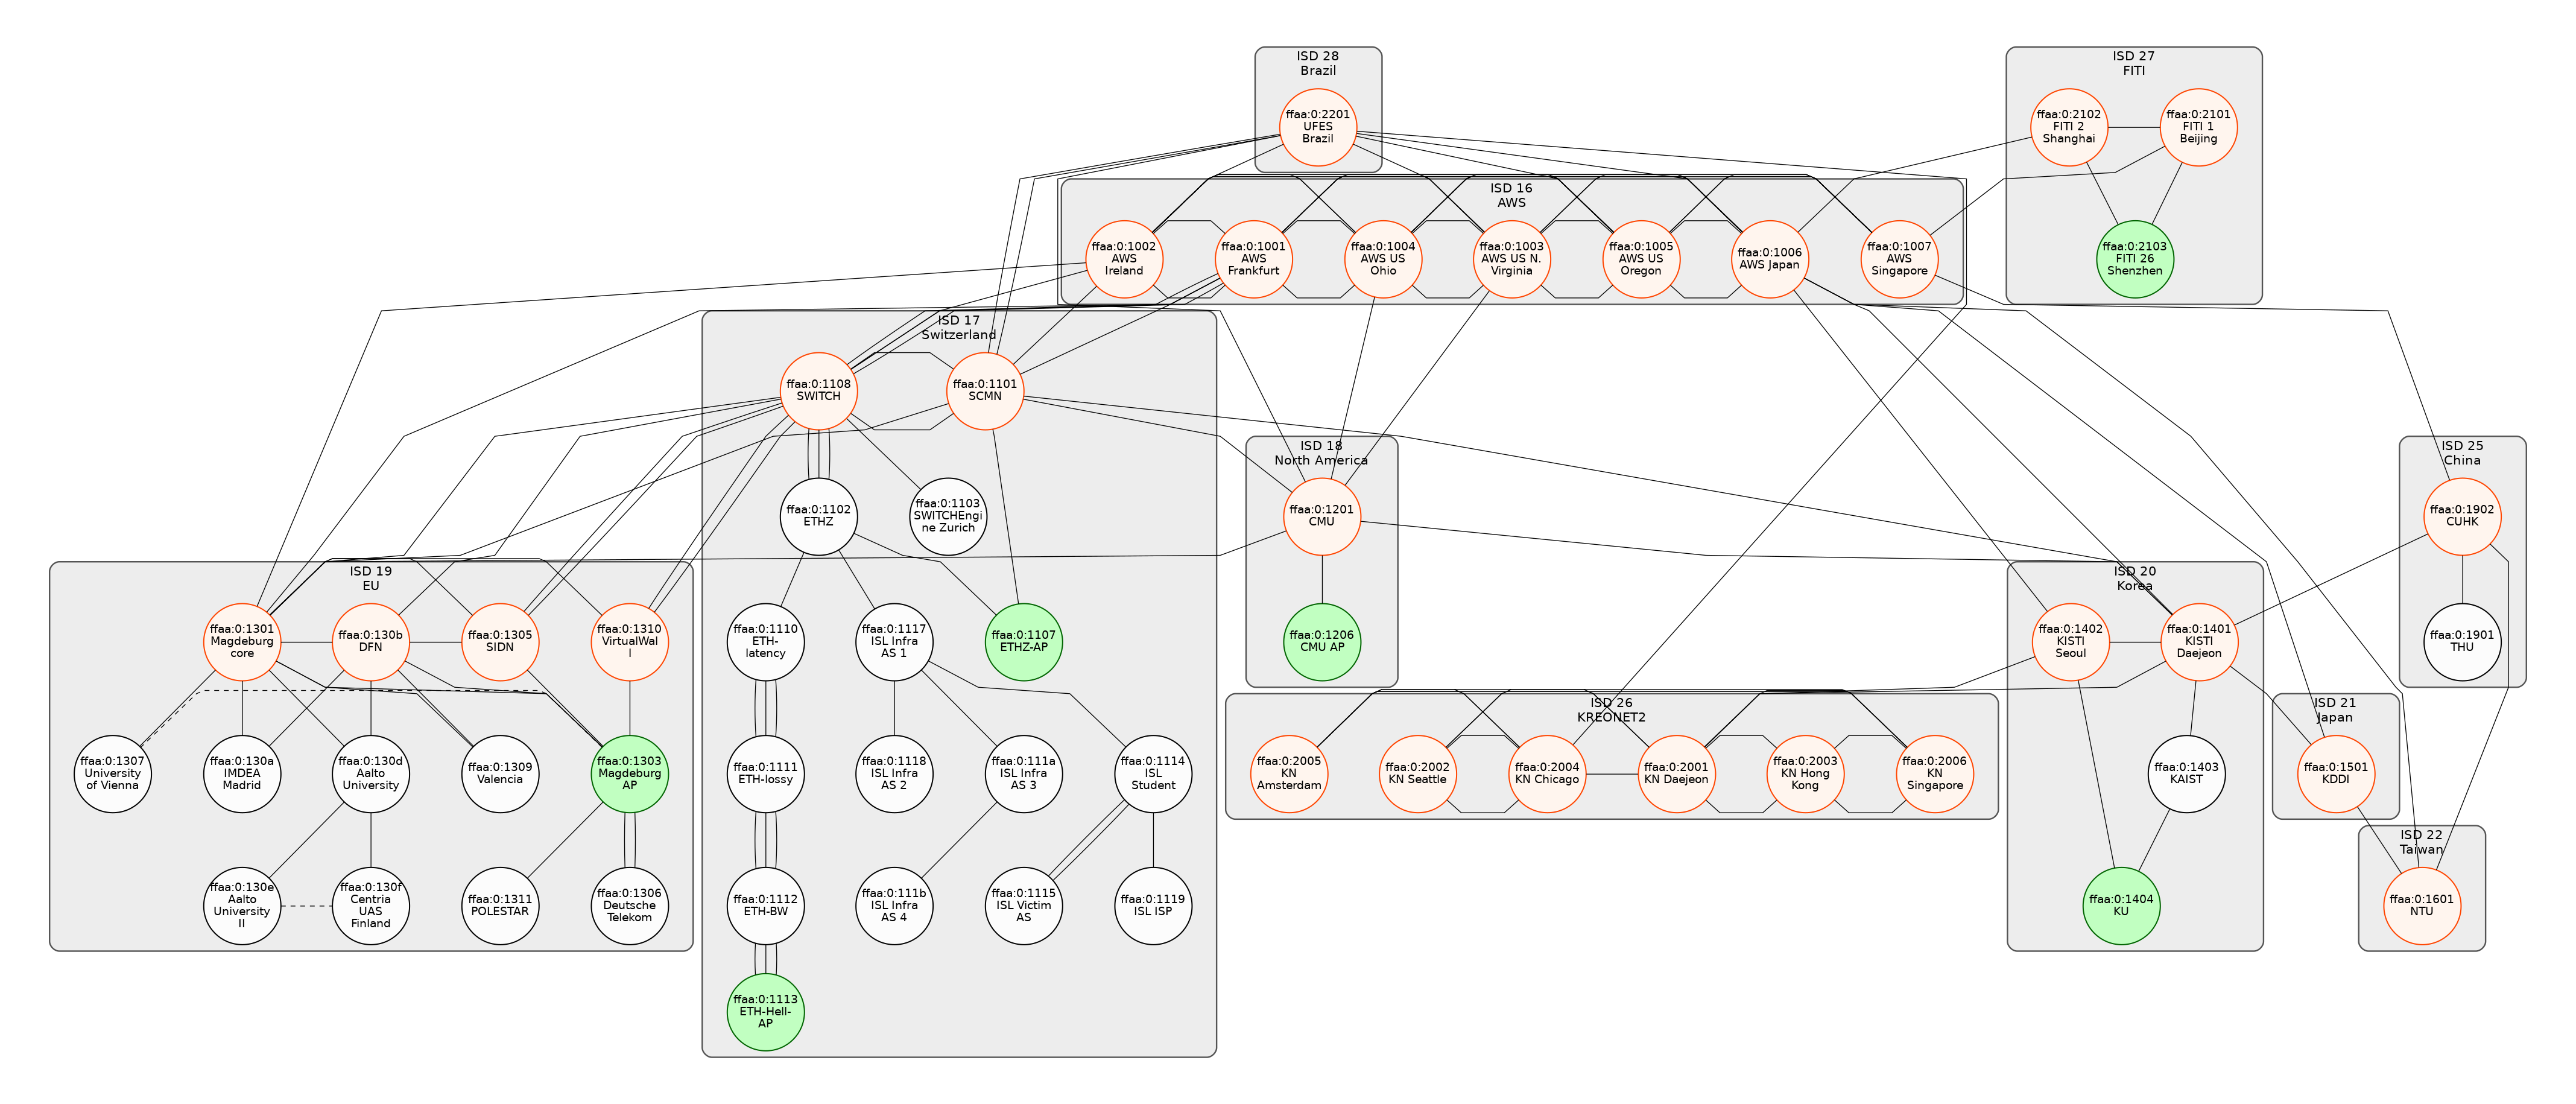
\includegraphics[width=\textwidth]{figures/Figure_1_ScionLabTopology.png}
      \caption{Overview of the SCIONLab testbed topology at the time of the measurement campaign. Vantage-point ASes were attached to ISD 17 (Switzerland), ISD 18 (United States), and ISD 19 (Europe). Not every AS shown was reachable throughout the four-week study; only persistently reachable ASes were retained for longitudinal analysis. Original image adapted from SCIONLab.org.}
      \label{fig:scionlab-topology}
    \end{figure}
    

\subsection{Measurement Suite}
    The measurement suite is a host-based, modular telemetry framework that operates entirely at the network edge. It interfaces with the standard SCION Dispatcher via UNIX domain sockets, thereby collecting both control-plane metadata (through the \texttt{scion showpaths} API) and data-plane performance metrics without requiring any in-network programmable hardware. This design enables Differential State Analysis: a direct quantitative comparison between the paths advertised by the control plane and the paths that are actually operational from the application's perspective.

    The suite is architected to decouple SCION-specific probing logic from network-agnostic data handling and analysis. All network-facing operations are encapsulated in five independent, reusable modules. Each module produces structured JSON output that is consumed by downstream modules or by the analysis pipeline. The five modules are:

    \begin{description}
        \item[Control-Plane Discovery Service (\texttt{pathdiscover})] This module periodically enumerates the complete set of available end-to-end paths between each directed AS-pair in the measurement mesh. It invokes the SCION control-plane API (\texttt{scion showpaths}) with appropriate source and destination AS identifiers and parses the returned path vectors. For every discovered path, the module extracts a unique path fingerprint (a canonical string representation of the sequence of ISD-AS-hop identifiers and interface numbers) together with metadata such as MTU, next-hop IP addresses, and any policy constraints. The resulting path set is written to a timestamped JSON file and serves as the authoritative ground truth for subsequent differential analysis.\\

        \item[Differential State Analyzer (\texttt{comparer})] This module performs a set-theoretic comparison between the path sets produced by consecutive executions of \texttt{pathdiscover}. Using the unique path fingerprints, it identifies three classes of events: (i) path births (new paths that appear in the current interval but were absent in the previous interval), (ii) path deaths (paths that disappear), and (iii) persistent paths (present in both intervals). Timestamps of birth and death events are recorded to compute path lifetime distributions and control-plane churn rates (i.e., the frequency and magnitude of path-set changes). These metrics quantify the stability of the SCION control plane over the four-week campaign.\\

        \item[Data-Plane Performance Prober (\texttt{prober})] For each measurement interval, this module samples up to 15 paths uniformly at random from the current discovery set for every destination AS, so that the single-path baseline is not biased toward any particular path property. It then establishes isolated sessions along each selected path and measures application-visible performance. The prober records round-trip time (RTT), jitter (standard deviation of RTT), and packet-loss ratio by transmitting 15 probe packets per path. This volume provides a stable estimate of RTT and loss while keeping the per-interval measurement load modest on the shared SCIONLab infrastructure. All measurements are performed sequentially to establish a clean baseline of single-path behavior before any concurrent usage is introduced.\\
        
        \item[Multipath Orchestration Evaluator (\texttt{mp-prober})] This module quantifies the performance impact of concurrent multipath transport. From the current discovery set it selects up to three paths at random and orchestrates simultaneous flows across them; the paths are not required to be strictly disjoint and may therefore share links or hops. The number of concurrent paths was limited to two or three (two for the bandwidth tests) to avoid overloading the shared SCIONLab infrastructure. The same performance metrics (RTT, jitter, packet loss) are collected for each constituent path while the flows run in parallel. By comparing these concurrent measurements against the single-path baseline obtained by \texttt{prober}, the module quantifies how per-path metrics differ between single-path and concurrent operation; as discussed in Section~\ref{sec::result}, the design does not allow such differences to be attributed to a specific cause such as shared links, end-host scheduling, or router load.\\

        \item[Capacity Verification Modules (\texttt{bw-alldiscover} and \texttt{bw-multipath})] These two modules perform active throughput measurements using the official \texttt{scion bwtestclient} tool. Each bandwidth measurement with \texttt{scion bwtestclient} was run for 3 seconds in each direction. The \texttt{bw-alldiscover} module first evaluates aggregate bandwidth across all discovered paths in isolation (single-path capacity). The \texttt{bw-multipath} module then repeats the tests while running up to two paths concurrently, thereby exposing directional bottlenecks and any performance difference relative to single-path operation. To avoid overloading the shared, non-production SCIONLab infrastructure, bandwidth tests were deliberately limited to a maximum of two concurrent paths per destination and were executed only after all lighter-weight latency and loss measurements had completed.\\
    \end{description}
    % All scripts output their raw data into dated directories for later use.
    All modules were executed in a strict sequential pipeline within each 30-minute cron invocation: discovery, differential analysis, single-path probing, multipath evaluation, and bandwidth verification. This ordering guarantees that every data-plane measurement is performed on a path set that has been freshly validated by the control plane.
    

\subsection{Analysis Suite}
    The analysis suite consists of a collection of scripts that ingest the raw JSON archives produced by the measurement modules. Processing occurs independently for each directed AS-pair. The pipeline extracts and computes the following core metrics for every measurement interval:
    \begin{itemize}
    \item Average, minimum, maximum, and 95th-percentile RTT;
    \item Jitter (standard deviation of RTT samples);
    \item Packet-loss ratio (percentage of probes lost);
    \item Path-churn statistics (number of births, deaths, and total path-set changes per day);
    \item Multipath degradation ratios (relative change in per-path metrics under concurrent usage);
    \item Aggregate bandwidth and directional bottleneck identification.
\end{itemize}
    Temporal aggregation is performed over the stable 27-day window (16 July to 11 August 2025). Outlier detection and missing-data imputation routines (based on median values from neighboring intervals) are applied where necessary to maintain continuity. The processed results are stored in compact summary tables that directly feed the visualizations and statistical tests presented in Section~\ref{sec::result}. All analysis code, together with the complete raw dataset, is available in the public repository~\cite{github-scionlab-data}.


\section{Results}~\label{sec::result}
This section presents the key findings from our four-week measurement campaign. A preliminary comparison across all three vantage points (attached to geographically distributed SCIONLab ISDs) revealed highly consistent trends in both control-plane dynamics and data-plane performance. For clarity and to avoid redundancy, the figures and primary quantitative analysis in this paper focus on data collected from a single representative vantage point (AS-1). Results from the other two vantage points show qualitatively similar patterns and are available in full in our public repository~\cite{github-scionlab-data}; for bandwidth, the upstream/downstream asymmetry holds at all three vantage points, but the absolute gap is smaller at the other two.

\subsection{Path Availability and Churn}
Our measurements demonstrate that the SCIONLab environment is characterized by substantial and continuous path churn. The set of available end-to-end paths between each directed AS-pair fluctuated constantly, with paths appearing and disappearing throughout the stable 27-day observation window (16 July to 11 August 2025). This dynamic behavior is illustrated in Figure~\ref{fig:churn-events}, which plots the number of paths added and removed in every 30-minute interval.

\begin{figure}[h!]
  \centering
  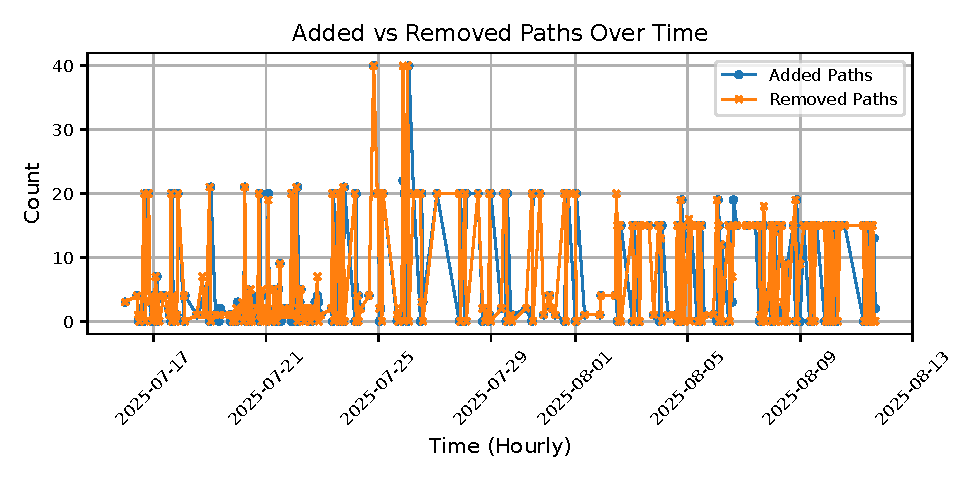
\includegraphics[width=\textwidth]{figures/1_Comparer/Figure_2_plot_add_remove_over_time.pdf}
  \caption{Path churn over the measurement period. The plot shows the number of paths added (positive) and removed (negative) between the representative vantage point and its two target destinations in each 30-minute interval.}
  \label{fig:churn-events}
\end{figure}

To quantify churn, we performed a pairwise set-theoretic comparison of path sets across the 1{,}281 consecutive 30-minute intervals. For the destination \texttt{17-ffaa:1:11e4} we observed 161 change events, involving 557 path additions and 577 path removals. This yielded an average path lifetime of 15.7~hours. Churn was even more pronounced toward \texttt{18-ffaa:1:11e5}, where 301 change events occurred, with 1{,}254 paths added and 1{,}259 removed, resulting in a markedly shorter average path lifetime of \textbf{8.6~hours}.

The additions and removals in Figure~\ref{fig:churn-events} are indeed correlated, but they are rarely path replacements: across the six directed vantage-point series, only 33 of 1{,}126 change events (2.9\%) contain both an addition and a removal in the same interval, and 99.6\% of all added paths had already been alive earlier in the window. Each directed pair lists only 18--24 distinct paths over the 27 days, so the churn consists mainly of the same paths being withdrawn and restored: toward \texttt{17-ffaa:1:11e4} and \texttt{18-ffaa:1:11e5}, 77\% and 88\% of the additions seen from the representative vantage point are the whole path set reappearing after an interval in which \texttt{scion showpaths} returned no viable path, and 97\% of the per-path timeout episodes (all six series) last a single 30-minute interval. The only change in path-set composition occurs on 2 August 2025 at 11:00, when the 9--11 paths traversing the ISD~16 core AS \texttt{16-ffaa:0:1001} are no longer listed (four paths via \texttt{20-ffaa:0:1401} appear at the same time for the pair involving ISD~18 and ISD~19); otherwise, the paths of a pair share the same first and last three ASes and differ only in the core transit segment (via ISD~16, ISD~20, or different ISD~17/19 core ASes) and in the interfaces used between them. These events appear in the path sets returned by the SCION control-plane API at all three vantage points, and the 127-interval outage of \texttt{17-ffaa:1:11e4} (9--11 August) is observed identically by all of them, so the churn is not specific to a single measurement VM. Most short-lived events, however, do not coincide across vantage points, so we cannot exclude that the local host or SCION daemon contributes to them.

The high frequency of these events is further highlighted in Figure~\ref{fig:change-events}, which shows that path-set changes occurred in the majority of observation intervals (intervals with zero changes are omitted for visual clarity).

\begin{figure}[h!]
  \centering
  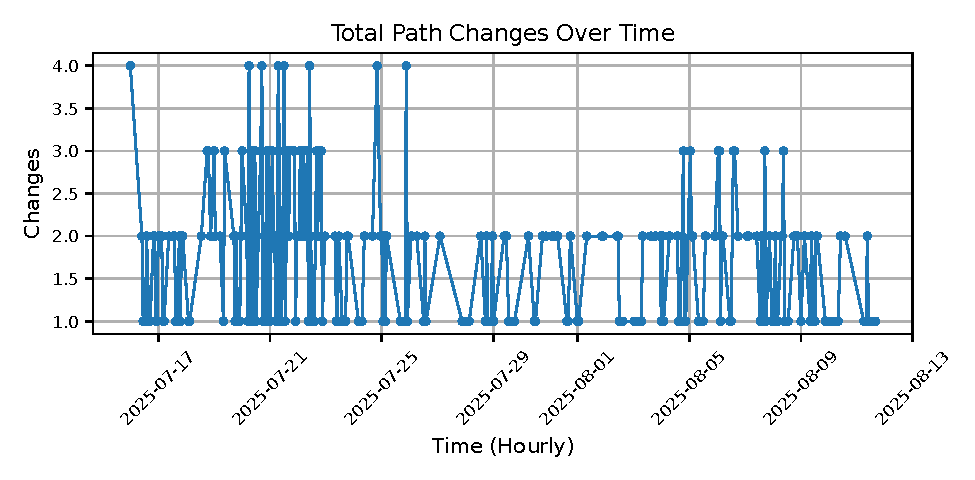
\includegraphics[width=\textwidth]{figures/1_Comparer/Figure_3_plot_path_changes_over_time.pdf}
  \caption{Frequency of path change events. Each point represents a 30-minute interval in which the set of available end-to-end paths changed relative to the preceding interval.}
  \label{fig:change-events}
\end{figure}

Consequently, the vast majority of paths proved ephemeral. The lifetime distribution in Figure~\ref{fig:lifetime-dist} reveals that most paths persisted for fewer than 100{,}000~seconds ($\approx$27.8~hours), confirming that long-lived paths are the exception rather than the rule in the current SCIONLab deployment. These churn rates imply that any path-scoring service relying on exponential moving averages of donated telemetry must refresh its view at a high cadence; otherwise the averages rapidly become stale.

\begin{figure}[h!]
  \centering
  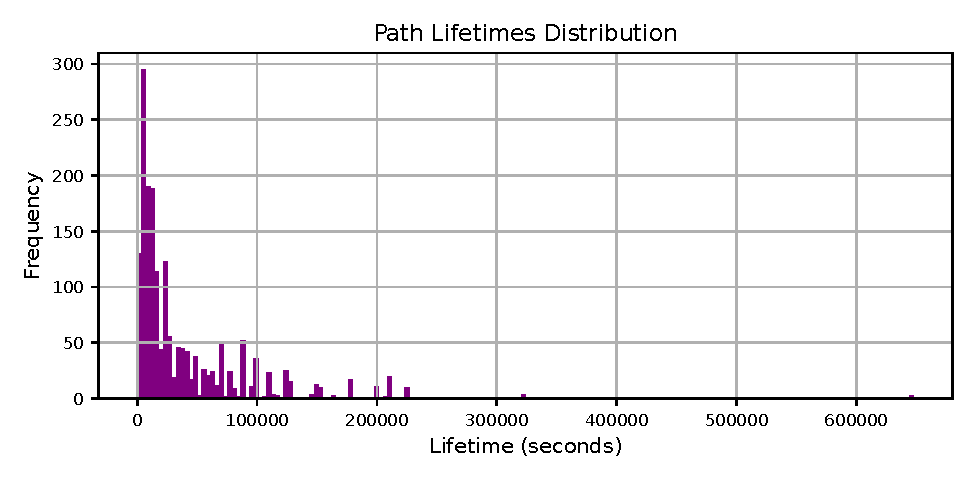
\includegraphics[width=\textwidth]{figures/1_Comparer/Figure_4_plot_path_lifetime_histogram.pdf}
  \caption{Distribution of individual path lifetimes across the entire campaign. The histogram uses 1-hour (3{,}600~s) bins and covers the full observed range (up to about 646{,}000~s).}
  \label{fig:lifetime-dist}
\end{figure}

\subsection{Latency and Loss Analysis}
Data-plane performance was evaluated by probing up to 15 randomly sampled paths per destination in each interval. Aggregated across the campaign, the two target ASes exhibited distinct performance profiles:

\begin{itemize}
    \item Paths toward \texttt{17-ffaa:1:11e4} showed a higher mean round-trip time (RTT) of 470.96~ms but lower packet loss of 0.36\%.
    \item Paths toward \texttt{18-ffaa:1:11e5} offered a lower mean RTT of 404.97~ms at the expense of higher packet loss (0.53\%).
\end{itemize}

The observed mean RTTs (approximately 405--471~ms) are high relative to typical Internet latencies. This is expected for the SCIONLab testbed, which operates as an overlay on the public Internet: end-to-end paths frequently traverse multiple Isolation Domains and may incur additional encapsulation or tunnel overhead. These figures should therefore be interpreted as characteristic of the current experimental deployment rather than of a native production SCION network.

Time-series analysis revealed a pronounced stabilization event around 2 August 2025. As shown in Figure~\ref{fig:rtt-over-time}, RTT values for both destinations became markedly less volatile after this date. This shift was observed uniformly across all three measurement ASes, suggesting a network-wide change in the SCIONLab topology. Notably, the latency stabilization did not coincide with improved reliability: packet-loss behavior (Figure~\ref{fig:loss-over-time}) remained highly erratic before and after the event. We hypothesize that the disappearance of several unstable, high-latency paths around 2 August was responsible for the observed RTT stabilization. We did not contact the SCIONLab maintainers about this event. The timing coincides with the disappearance of the paths that traversed the ISD-16 core AS (\texttt{16-ffaa:0:1001}), which we observed in the control-plane data; we therefore hypothesize that the removal of these higher-latency paths produced the observed RTT stabilization.

\begin{figure}[h!]
  \centering
  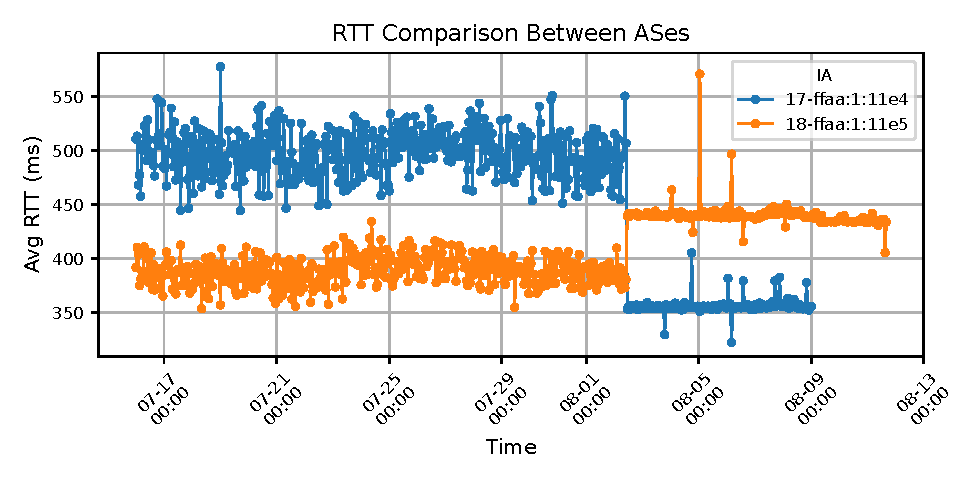
\includegraphics[width=\textwidth]{figures/2_Prober/Figure_5_combined_rtt_plot.pdf}
  \caption{Time series of average round-trip time (RTT) to both target ASes. A clear stabilization and downward shift in latency occurs around 2 August 2025.}
  \label{fig:rtt-over-time}
\end{figure}

\begin{figure}[h!]
  \centering
  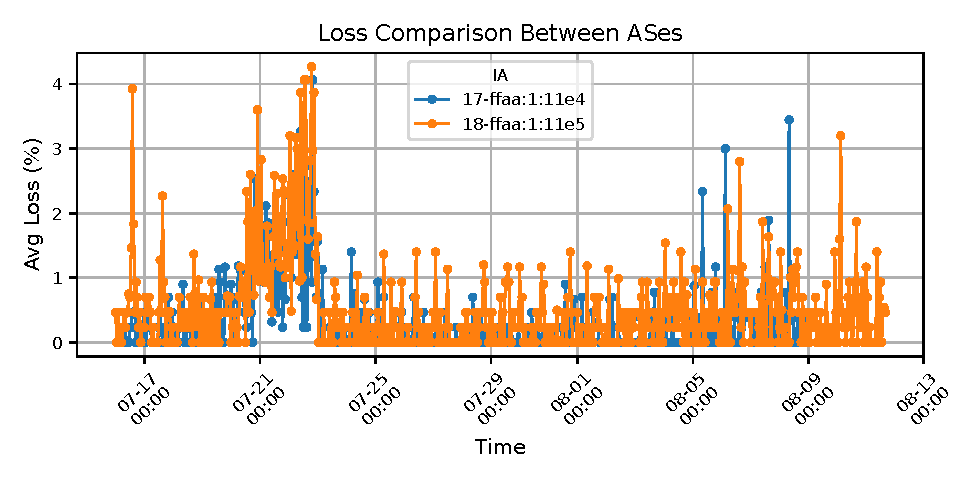
\includegraphics[width=\textwidth]{figures/2_Prober/Figure_6_combined_loss_plot.pdf}
  \caption{Time series of average packet-loss ratio to both target ASes. In contrast to RTT, packet loss exhibits no corresponding stabilization.}
  \label{fig:loss-over-time}
\end{figure}

\subsection{Bandwidth Performance Asymmetry}
Active throughput measurements using the \texttt{scion bwtestclient} at the 100~Mbps tier exposed a striking directional asymmetry. Downstream (server-to-client) traffic achieved consistently high utilization, while upstream (client-to-server) traffic was severely constrained.

\begin{itemize}
    \item \textbf{Downstream ($S \rightarrow C$)}: Average achieved throughput was 87.09~Mbps, with an average loss ratio of 12.9\% (again reflecting an offered load above the available capacity, but far less severe than in the upstream direction).
    \item \textbf{Upstream ($C \rightarrow S$)}: Average throughput dropped to 65.4~Mbps, accompanied by extremely high and volatile packet loss averaging \textbf{34.6\%} (see Figure~\ref{fig:bw-loss-cs}). The reported 34.6\% packet loss is the average loss ratio returned by \texttt{scion bwtestclient} (over 1{,}306 completed single-path tests toward the 18-ffaa:0:1201 server) when the client attempted to send at the configured 100~Mbps tier. Because the available upstream capacity was lower than the offered load, a substantial fraction of packets were dropped; the loss figure therefore reflects capacity mismatch rather than random background loss.
\end{itemize}

This persistent upstream degradation is consistent with systemic bottlenecks or restrictive forwarding policies within the SCIONLab testbed infrastructure.

These averages were representative of the whole campaign (Figure~\ref{fig:bw-time-series}): toward the 18-ffaa:0:1201 server, the daily mean downstream throughput stayed between 82.4 and 88.4~Mbps and the daily mean upstream throughput between 53.6 and 68.4~Mbps, with weekly means of 86.0--87.8~Mbps and 63.7--67.0~Mbps, respectively. The terms client and server refer to the roles assigned by \texttt{scion bwtestclient} in each directed test: the client is the vantage-point AS that initiates the test, and the server is a SCIONLab bandwidth-test server (18-ffaa:0:1201 or 19-ffaa:0:1303) rather than another vantage point, so upstream and downstream denote the direction relative to the vantage point. The upstream throughput follows directly from the loss: under a 100~Mbps offered load, the measured throughput is consistent with $100 \times (1 - 0.346) \approx 65.4$~Mbps, since only packets that arrive are counted as achieved throughput.

\begin{figure}[h!]
  \centering
  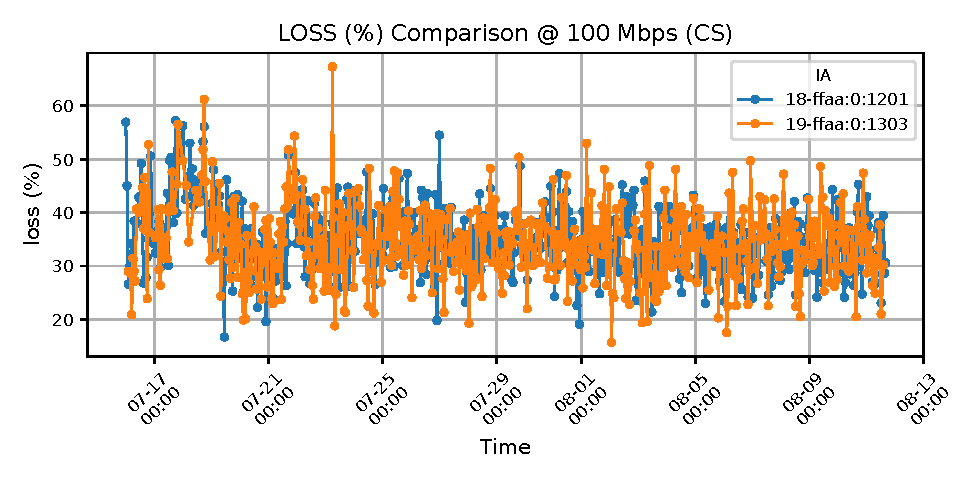
\includegraphics[width=\textwidth]{figures/3_Bandwidth/Figure_7_tier_100_cs_loss_per_IA.pdf}
  \caption{Upstream (client-to-server) packet-loss ratio at the 100~Mbps tier. The plot reveals persistently high and volatile loss, confirming a severe directional bottleneck.}
  \label{fig:bw-loss-cs}
\end{figure}

\begin{figure}[h!]
  \centering
  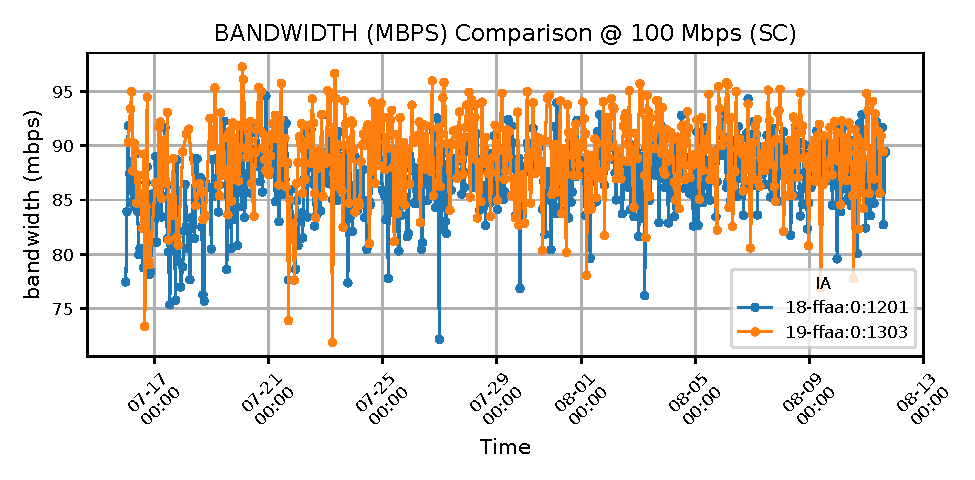
\includegraphics[width=\textwidth]{figures/3_Bandwidth/Figure_7b_tier_100_sc_bandwidth_per_IA.pdf}
  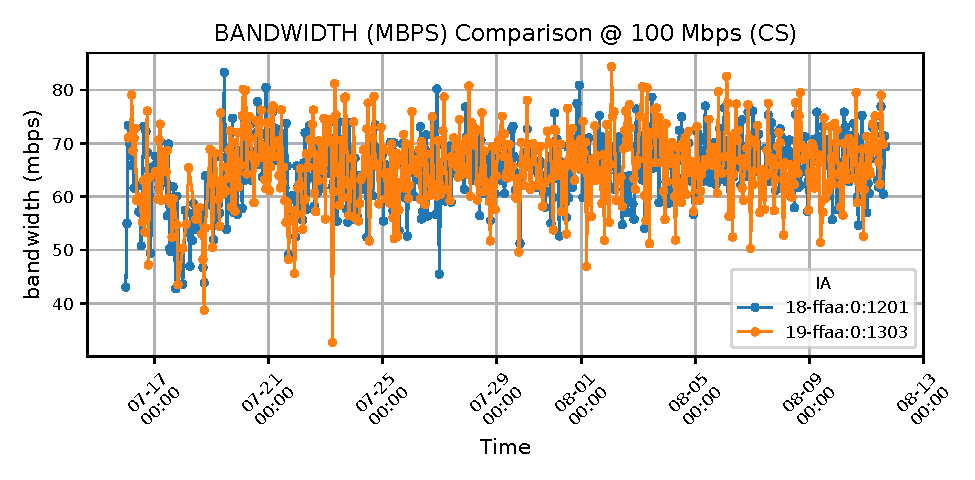
\includegraphics[width=\textwidth]{figures/3_Bandwidth/Figure_7c_tier_100_cs_bandwidth_per_IA.pdf}
  \caption{Hourly mean achieved throughput at the 100~Mbps tier over the 27-day window, measured from the vantage point AS-1 toward the two bandwidth-test servers. Top: downstream (server-to-client). Bottom: upstream (client-to-server).}
  \label{fig:bw-time-series}
\end{figure}

\subsection{Single-Path versus Multipath Performance Trade-offs}
To evaluate the impact of concurrent multipath usage, we compared performance metrics for each path when used in isolation (Single-Path, SP) versus when probed concurrently with up to two other paths (Multipath, MP). In the SP probes, one randomly sampled path at a time is probed with 15 pings; roughly seven minutes later, the MP prober pings up to three paths concurrently (15 pings each), drawn at random from the current path set to the same destination and not constrained to be disjoint. We pair every SP probe with an MP probe of the same path (identified by its fingerprint) taken within 15 minutes of it, and compute the difference MP minus SP of the mean RTT, of the jitter (the \texttt{mdev} statistic that \texttt{scion ping} reports over the 15 echo replies), and of the packet-loss ratio (in percentage points; one lost reply corresponds to 6.7 points). Positive differences therefore indicate worse performance under multipath. We test each metric with a paired Wilcoxon signed-rank test and report the median difference and the matched-pairs rank-biserial correlation $r$ as effect size. Because probe pairs from the same path are not independent, we report the test both over all probe pairs and over the 44 per-path median differences.

For the 19-ffaa:1:11de vantage point this yields 5,792 probe pairs over 44 paths. Figure~\ref{fig:sp-mp-latency} shows that the distributions of the differences are centered on zero and do not support a blanket degradation of the per-path metrics. The median RTT difference is $-0.05$~ms (interquartile range $-1.06$ to $+1.27$~ms; Wilcoxon $p=0.78$, $r=0.004$), and the RTT is lower under multipath in 52\% of the pairs; the per-path medians show the same picture ($-0.10$~ms, $p=0.58$). For jitter, the median difference is $+0.06$~ms ($r=0.08$); this is statistically significant over probe pairs ($p<10^{-6}$) but practically negligible, and not significant over the 44 per-path medians ($+0.04$~ms, $p=0.07$). The mean jitter difference ($+1.3$~ms) exceeds the median because of a heavier upper tail: the 95th percentile of the difference is $+12.7$~ms, compared with $-8.7$~ms for the 5th percentile. Packet loss is identical in 92\% of the pairs; multipath loss is higher in 4.9\% and lower in 3.4\% of the pairs (mean difference $+0.24$ percentage points, $p=3\times10^{-6}$ over probe pairs, $r=0.23$), while the median difference is zero for every one of the 44 paths, so no per-path test is possible. The other two vantage points show the same qualitative picture (median RTT differences between $-0.14$ and $-0.05$~ms, median jitter differences between $+0.06$ and $+0.19$~ms, and zero median loss difference); at the path level their RTT differences are significant, but in the direction of slightly lower RTT under multipath. Overall, we observe no change in typical per-path latency under concurrent usage, only a modest increase in the upper tail of the jitter distribution and a small excess of loss events. Because the SP and MP probes are not simultaneous and the tails extend in both directions, these data do not allow us to attribute the tail effect to resource contention at end hosts or shared bottleneck links; isolating that cause would require simultaneous, controlled measurements.

\begin{figure}[h!]
  \centering
  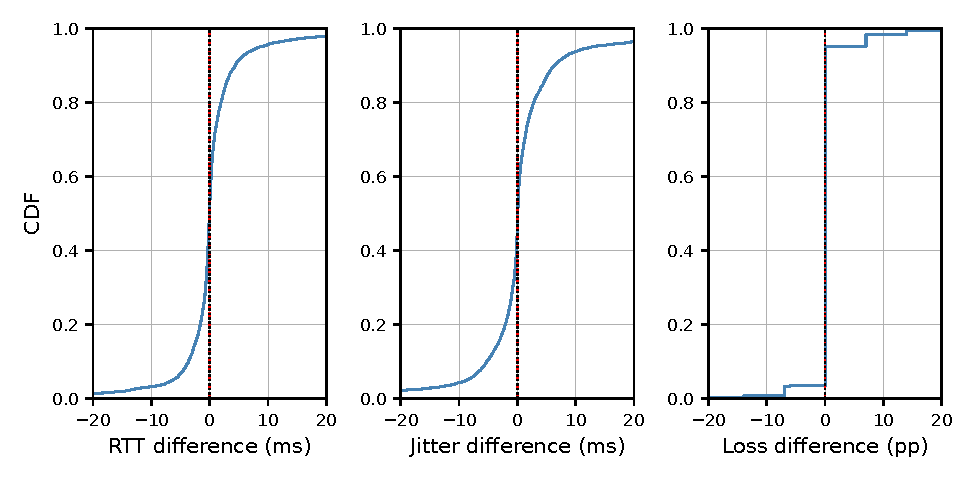
\includegraphics[width=0.9\linewidth]{figures/4_SP-MP-Prober/Figure_8_sp_mp_diff_cdf.pdf}
  \caption{CDFs of the per-probe-pair differences (MP minus SP) in mean RTT, jitter, and packet-loss ratio for the 19-ffaa:1:11de vantage point (5,792 pairs, 44 paths). Positive values indicate worse performance under concurrent multipath usage. The dashed red line marks zero and the dotted black line marks the median. Axes are truncated at $\pm20$; this hides 3.5\% of the RTT, 5.8\% of the jitter, and 0.3\% of the loss differences.}
  \label{fig:sp-mp-latency}
\end{figure}

Aggregate throughput, in contrast, increased substantially in multipath mode. As shown in Figure~\ref{fig:sp-mp-bandwidth}, while individual path bandwidths varied, the combined throughput of the multipath session consistently exceeded that of any single path. This establishes a trade-off in the current SCIONLab environment: applications obtain significantly higher total bandwidth at little cost in median per-path latency, but with a heavier jitter tail and occasional additional loss. These findings suggest that future multipath schedulers (e.g., for Multipath QUIC) could take the heavier jitter tail into account when placing latency-sensitive flows, while multiplexing bulk transfers across multiple paths.

\begin{figure}[h!]
  \centering
  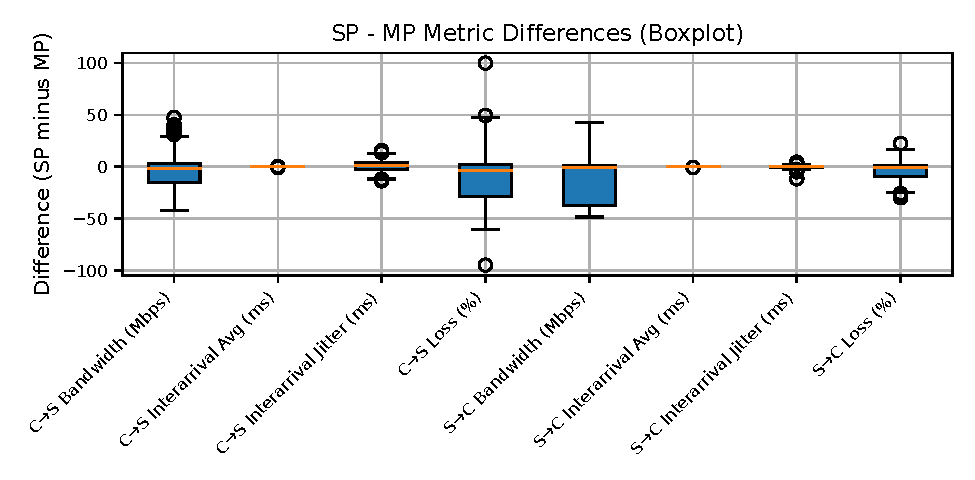
\includegraphics[width=0.9\linewidth]{figures/5_SP-MP-bw/Figure_9_sp_mp_bw_diff_boxplot.pdf}
  \caption{Performance differences for bandwidth metrics (SP minus MP). Although per-path throughput is mixed, aggregate multipath throughput is consistently higher.}
  \label{fig:sp-mp-bandwidth}
\end{figure}

Our prober samples paths uniformly at random, whereas a real endpoint is likely to prefer low-latency paths. To gauge the difference, we compare, in each measurement interval, the average RTT of the up to 15 sampled paths with the lowest average RTT among them (vantage point 19-ffaa:1:11de). Toward \texttt{17-ffaa:1:11e4}, the median across intervals is 484~ms for the average and 263~ms for the minimum; toward \texttt{18-ffaa:1:11e5}, it is 400~ms and 265~ms, so the best sampled path is typically 33--45\% faster than the average path (the other two vantage points show similar gaps, with medians of 98--219~ms). By contrast, the gap between the average and the minimum RTT of the 15 pings on a single path is small (median 1.5~ms). The mean RTTs reported above therefore describe a randomly chosen path and overstate what a latency-aware endpoint would experience, and our random-sampling results are a baseline rather than the outcome of an optimized selection policy. Since at most 15 paths are probed per interval, the minimum is only an upper bound on the best RTT available in the full path set.


\subsection{Path Discrepancy: Asymmetric Path Discovery}
Our measurements revealed the phenomenon of \textit{path discrepancy}, in which the set of available end-to-end paths between two ASes is not symmetric. For example, during multiple intervals AS-3 discovered 20 viable paths toward AS-2, while AS-2 simultaneously discovered only 18 viable paths in the reverse direction toward AS-3.
To quantify this effect, we compared the number of viable (non-timeout) paths discovered in the two directions between each pair of vantage-point ASes (AS-1, AS-2, AS-3) in every 30-minute interval of the stable 27-day window; of the 3{,}840 pairwise comparisons, 402 were excluded because at least one direction returned an empty path set (in the 140 cases where only one direction did, the difference was up to 20 paths).
Across the remaining 3{,}438 intervals, the forward and reverse path-set sizes differed in 1{,}088 (31.6\%); the mean absolute difference was 0.63 paths (median 0), rising to a mean and median of 2 paths in the intervals where a difference occurred, and the maximum difference was 8 paths.
The discrepancy was concentrated in the AS-2/AS-3 pair, whose path-set sizes differed in 852 of 1{,}147 intervals (74.3\%) and was larger at AS-3 in 829 of them (97.3\%), indicating a consistent directional bias, whereas the pairs involving AS-1 differed in 6.4\% and 13.9\% of intervals with no consistent direction.
The 20-versus-18 configuration described above occurred in 730 intervals between 16 July and 2 August, after which both directions typically reported nine paths.
When timed-out paths are also counted, the AS-1 pairs show no differences at all, and the AS-2/AS-3 pair differs in 835 intervals by exactly two paths, always with the larger set at AS-3; the differences involving AS-1 therefore reflect path liveness rather than differing sets of discovered paths.
% 
This asymmetry is not a transient failure but an expected consequence of SCION's path-aware design. Each autonomous system retains full administrative autonomy over the path segments it accepts and advertises; forward- and reverse-path availability are therefore independently determined by local policies. As a direct result, path verifiability is inherently directional.

For management frameworks such as PoT-PolKA~\cite{borges2024pot}, which rely on in-situ telemetry to verify compliance with service-level agreements (SLAs), this discrepancy has important consequences: a successfully verified forward path provides no guarantee of a viable reverse path for control-plane feedback or acknowledgments. Consequently, SLAs in path-aware networks must be specified, monitored, and enforced as independent unidirectional entities rather than assuming symmetric bidirectional flows.
% 
The same observation carries direct implications for multipath transport protocols such as Multipath QUIC. While modern multipath protocols such as Multipath QUIC validate a path in both directions before use and can transmit acknowledgments on any validated path, the systematic discrepancy we observe still means that a path discovered and validated by one endpoint is not guaranteed to be available or high-quality for the peer. The same directional asymmetry also affects unipath protocols that rely on reverse-path feedback. Accounting for path discrepancy is therefore essential for any application or management system that requires reliable bidirectional consistency.

\section{Discussion}~\label{sec::discussion}
Our four-week longitudinal study provides the first large-scale empirical characterization of path dynamics in a live path-aware network. By continuously enumerating control-plane paths, probing data-plane performance, and contrasting single-path versus concurrent multipath operation, we expose three interlocking operational realities that must inform the design of both network management systems and transport protocols: (1) substantial and frequent path-set churn, (2) systematic path discrepancy, and (3) a throughput gain accompanied by only a modest increase in the jitter tail and a small excess of loss events under multipath usage. By quantifying these phenomena with high temporal resolution, our work establishes the empirical boundary conditions for autonomous lifecycle management in path-aware networks (PANs) and supplies the evidence-based foundation required to refine next-generation multipath transport protocols. The path-churn rates we measure directly affect the practicality of host-driven path selection and automated orchestration: a scoring or selection service whose view of the path set is more than a few hours old risks recommending paths that have already disappeared.

First, the observed control-plane churn—with average path lifetimes as short as 8.6~hours—fundamentally challenges the reliability of dynamic path-scoring services such as the Path Oracle~\cite{kruger2023path}. These services rely on exponential moving averages of donated telemetry, yet in an environment where more than half the available paths can appear or disappear within a single 30-minute interval, historical averages rapidly become stale. Management planes must therefore transition from long-term averaging to high-cadence, real-time telemetry collection to maintain an accurate network view. For multipath transport protocols such as Multipath QUIC~\cite{ietf-quic-multipath-15} and DMTP~\cite{john2023dmtp}, this churn implies that schedulers cannot treat the path set as quasi-static; they must incorporate continuous low-overhead probing and rapid failover, elevating path stability to a first-order selection criterion alongside latency and bandwidth.

An average path lifetime of 8.6--15.7~hours is indeed sufficient for the majority of short-lived request-response exchanges. However, the same lifetime is short relative to the timescales assumed by long-lived transport connections, by path-scoring services that maintain exponential moving averages of donated telemetry, and by automated SLA-verification systems that treat a discovered path as a stable entity. In these settings the observed churn rate directly determines how frequently path sets and path scores must be refreshed.

Second, the phenomenon of path discrepancy—where the set of viable paths from A to B differs from the set from B to A—challenges the bidirectional symmetry that conventional network management and transport design have traditionally taken as a working assumption, even though Internet routes are often asymmetric~\cite{paxson1997end}. Because each SCION autonomous system independently controls which path segments it accepts and advertises, forward- and reverse-path availability are policy-dependent and not guaranteed to match. This asymmetry compels management frameworks such as MS4PAN~\cite{boldrini2024ms4pan} to perform independent directional scoring when verifying true bidirectional service-level agreements (SLAs). Even for protocols such as Multipath QUIC, which validate paths in both directions and can acknowledge on any validated path, a path validated by one endpoint is not guaranteed to be available or high-quality for the peer, and the same asymmetry affects unipath protocols that rely on reverse-path feedback. Traffic-engineering policies must therefore become explicitly direction- and packet-size-aware, as our measurements confirm that upstream flows can suffer packet-loss rates exceeding 34\% even when downstream flows remain stable.

Third, concurrent multipath usage reveals a performance trade-off: while aggregate throughput increases substantially, we observe a modest increase in the tail of the jitter distribution and a small excess of loss events, with no change in typical RTT. Our measurements do not allow us to attribute this tail effect to a specific cause such as contention at end-host resources or shared bottleneck links. This trade-off poses an optimization problem for intent-based networking orchestration engines, which must decide, on a per-application basis, whether the throughput gain justifies the somewhat heavier jitter tail and occasional additional loss. Scheduler designs for Multipath QUIC and high-speed bulk-transfer systems such as Hercules~\cite{gartner2023hercules} can exploit this insight by adopting differentiated strategies, routing latency-sensitive control traffic over a single high-quality path while distributing throughput-oriented flows across multiple paths, rather than treating all paths equally.

Taken together, these findings demonstrate that autonomous lifecycle management in PANs cannot inherit the relatively static assumptions of BGP-based Internet operation. Instead, management planes must be engineered from the ground up for high volatility, inherent asymmetry, and explicit performance trade-offs. The measurement framework and public dataset we release with this work enable reproducible validation of these dynamics and lay the foundation for future comparative studies in production-grade SCION environments (e.g., SCIERA).

Several factors likely contribute to the phenomena we report. The high control-plane churn is consistent with SCION's beaconing process and with the experimental nature of the SCIONLab testbed, in which path segments are frequently refreshed or temporarily unavailable. The elevated RTTs and the strong upstream bandwidth asymmetry are characteristic of an overlay deployment running atop the public Internet, where encapsulation, multi-ISD transit, and shared underlay capacity can introduce both latency and directional bottlenecks. The modest multipath tail effects are consistent with occasional contention, although our non-simultaneous probing design does not allow us to isolate the precise location of that contention.

\paragraph{Limitations and Future Directions}
We emphasize that our measurements were conducted on the SCIONLab testbed, an experimental overlay network running atop the public Internet. Consequently, certain observed artifacts (particularly the severe upstream packet loss) may be influenced by underlying VPN tunnels or cloud-provider transit rather than being fundamental to the SCION architecture itself. In addition, our measurement suite interacts with the network through the standard SCION reference implementation, using UNIX-domain sockets to interface with the Dispatcher and UDP sockets for actual data-plane transmission. This software-level processing introduces additional overhead compared with optimized kernel-bypass solutions such as xiondp. Our multipath evaluation compares single-path and concurrent probe measurements rather than a full multipath transport session; a production multipath protocol could exhibit different scheduler and congestion-control interactions.

These results should therefore be interpreted as a foundational characterization of a developmental path-aware network rather than the definitive performance of a future production-grade SCION Internet. The next critical step is to redeploy the identical measurement framework in operational environments such as SCIERA. Such comparative studies will allow researchers to disentangle the intrinsic properties of SCION's architecture from implementation-specific artifacts of the current testbed.

\section{Conclusions}~\label{sec::conclusion}
In this paper we presented a four-week longitudinal measurement study of the SCIONLab testbed that provides the first comprehensive empirical characterization of operational dynamics in a deployed path-aware network. Our findings reveal a highly volatile environment governed by three fundamental properties: (1) significant control-plane churn, with average path lifetimes as short as 8.6~hours; (2) path discrepancy, an inherent asymmetry in path availability driven by independent AS policies; and (3) a performance trade-off in which concurrent multipath usage improves aggregate throughput at the cost of a modest increase in the tail of jitter and a small excess of loss events, with no change in typical RTT.

Collectively, these results supply the empirical ground truth required to move from experimental path-awareness to operational accountability and transparency in the Responsible Internet. They further demonstrate that next-generation multipath protocols such as Multipath QUIC must be explicitly designed to accommodate high churn and directional asymmetry. By releasing both the measurement framework and the complete raw dataset, we provide the community with the architectural constraints and reproducible data necessary for the development of SLA-verification frameworks, self-healing management planes, and robust multipath schedulers—thereby challenging the assumptions of path stability and symmetry inherited from the traditional Internet.

\backmatter


\section*{Declarations}

\subsection{Author Contributions}
\textbf{Lars Herschbach}: Conceptualization, Methodology, Software, Data curation, Formal analysis, Visualization, Writing -- original draft, Writing -- review \& editing.\newline
\textbf{Damien Rossi}: Software, Resources, Validation. \newline
\textbf{Sina Keshvadi}: Supervision, Methodology, Validation, Writing -- review \& editing. \newline

\subsection{Affiliation}
All work was carried out at TRU as part of the MITACS GRI program.

\subsection{Data Availability}
The datasets and analysis scripts generated during and/or analyzed during the current study are available in an online Github repository https://github.com/Keshvadi/mpquic-on-scion-ipc/


\subsection{Funding}
This research received no specific grant from funding agencies in the public, commercial, or not-for-profit sectors. Lars Herschbach and Damien Rossi were part of the Mitacs GRI internship Program which funded their stay in Canada. No Mitacs funding was intended for, or used in, the creation of this paper.
We would also like to thank Google for providing us with Google cloud credits making the persistent measurements using their infrastructure possible. 

\subsection{Competing Interests}
The authors declare that they have no known competing financial interests or personal relationships that could have appeared to influence the work reported in this paper.

\subsection{AI use statement}
The authors used OpenAI's ChatGPT to assist in language editing and structuring of the manuscript as well as in the creation of the measurement and analysis scripts. The authors reviewed, verified, and edited the content, and take full responsibility for its content.

% \noindent
% If any of the sections are not relevant to your manuscript, please include the heading and write `Not applicable' for that section. 






%%=============================================%%
%% For submissions to Nature Portfolio Journals %%
%% please use the heading ``Extended Data''.   %%
%%=============================================%%

%%=============================================================%%
%% Sample for another appendix section			       %%
%%=============================================================%%

%% \section{Example of another appendix section}\label{secA2}%
%% Appendices may be used for helpful, supporting or essential material that would otherwise 
%% clutter, break up or be distracting to the text. Appendices can consist of sections, figures, 
%% tables and equations etc.

\bibliographystyle{bst/sn-basic}
\bibliography{main}% common bib file


\end{document}
